\documentclass[a4paper,12pt, english]{article}
\usepackage[T1]{fontenc}
\usepackage[utf8]{inputenc}
\usepackage{graphicx}
\usepackage{babel}
\usepackage{amsmath}
\usepackage{ulem}
\usepackage{a4wide}
\usepackage{graphicx}
\usepackage{listings}
\usepackage{tabularx}
\usepackage{tabulary}

\title{FYS3150 - Prosjekt 2}
\author{John-Anders Stende}

\begin{document}

\section*{Introduction}

The aim of this project is to develop a code for simulating the solar system using the Runge-Kutta-4 (RK4) algorithm.

I will do this gradually by first setting up the coupled differential equations for the two-body problem Sun-Earth. These equations then need to be discretized and implemented in an RK4 solver. To test the RK4 algorithm I will compare the results to known closed-form solutions to this problem for different time steps $h$ 

Adding Jupiter results in a three-body problem. The differential equations for Earth then needs to be rewritten to account for the gravity of one more object. The aim of this set-up is to investigate how Jupiter alters Earth's orbit around the Sun. I will also discuss the stability of the RK4 solver when Jupiter's mass is increased for different $h$.

Finally, I will add the seven other planets to simulate the solar system and compare the results with the earlier problems. 

\section*{Runge-Kutta-4 algorithm}

RK4 is an iterative algorithm that approximates solutions to ordinary differential equations. It is based on Taylor expansion like Euler's method, but uses intermediate steps to find the slope when computing the next function value. These intermediate values are however computed with Euler's method. Consider the following definitions:
\[
\frac{dx}{dt}=f(t,x), \ x(t)=\int f(t,x)dt
\]
and discretized
\[
x_{i+1} = x_i + \int_{t_i}^{t_{i+1}}f(t,x)dt
\]
The latter equation is a discretized version of the Taylor expansion
\[
x(t+h) = x(t) + hf(t,x)
\]
If we simply set $f(t,x) = dx/dt$ we have Euler's method. RK4 however, computes the integral of $f(t,x)$ using Simpson's method:
\[
\int_{t_i}^{t_{i+1}}f(t,x)dt = x_i + \frac{h}{6} \lbrack f(t_i,x_i) + 2f(t_i+h/2,x_{i+1/2}) +
2f(t_i+h/2,x_{i+1/2}) + f(t_i+h,x_{i+1}) \rbrack
\]
\[
= x_i + \frac{h}{6} (k1 + 2k2 + 2k3 + k4)
\]
thus RK4 computes four different slopes $k_i$ and uses a weighted average of these to compute $x_{i+1}$. RK4 can be viewed as a predict-and-correct algorithm. We first compute a slope $k_1$ and use this to predict $x_{i+1/2}$ with Euler's method. This value is used to compute a new slope $k_2$, and then we use this new slope to correct $x_{i+1/2}$ with Euler's method, and so on. The idea is to compute the slope at different places in the interval $\lbrack t_i,t_{i+1} \rbrack$ to obtain a final slope that fits the function $x(t)$ we want to find better.

\section*{Two-body problem Sun-Earth}

The only force in this problem is gravity, given by Newton's law of gravitation
\[
F=\frac{GM_{\mathrm{Sun}}M_{\mathrm{Earth}}}{r^2},
\]
where $M_{\mathrm{sun}}$ is the mass of the Sun and $M_{\mathrm{Earth}}$ is the mass of Earth. $G$ is the gravitational constant and $r$ is the distance between Earth and the Sun.

I will account for both the Sun and Earth's motion while placing the Sun in the center-of-mass position, the origin. This is almost equivalent with neglecting the Sun's motion because $M_{\mathrm{Sun}} >> M_{\mathrm{Earth}}$. To keep the center-of-mass fixed, I set the Sun's initial velocity so that the total linear momentum of the two-body system is zero.

I assume that the orbit of Earth around the Sun is co-planar, and I take this to be the $xy$-plane. Using Newton's second law of motion we get the following equations for Earth:
\[
\frac{d^2x}{dt^2}=\frac{F_x}{M_{\mathrm{Earth}}},
\]
and 
\[
\frac{d^2y}{dt^2}=\frac{F_y}{M_{\mathrm{Earth}}},
\]
where $F_x$ and $F_y$ are the $x$ and $y$ components of the gravitational force. The equations for the Sun can be obtained by replacing $M_{\mathrm{Earth}}$ with $M_{\mathrm{Sun}}$ in the following. 

The next step is to rewrite these second-order differential equations as a set of coupled first order differential equations in the following way:
\[
\frac{dx}{dt}=v_x, \ \frac{d^2x}{dt^2}=\frac{dv_x}{dt}=\frac{F_x}{M_{\mathrm{Earth}}},
\]
and
\[
\frac{dy}{dt}=v_y, \ \frac{d^2y}{dt^2}=\frac{dv_y}{dt}=\frac{F_y}{M_{\mathrm{Earth}}},
\]
where component-wise F is obtained like this:
\[
F_x = -\frac{GM_{Sun}M_{Earth}cos\theta}{r^2} = -\frac{GM_{Sun}M_{Earth}rcos\theta}{r^3} = 
-\frac{GM_{Sun}M_{Earth}x}{r^3}
\]
where $r=\sqrt{x^2+y^2}$. The equation for $F_y$ is obtained by replacing $x$ with $y$. The negative sign ensures that the $F$ from the Sun on Earth acts in the negative $x$-direction when $x_{Earth}$ is positive and vice versa.

Standard units become very impractical when simulating the solar system because the model we use span many years and large distances. I will therefore use the astronomical unit 
($1 AU = 1.5x10^{11} m$) instead of meters and years ($1 yr = 3.2x10^7 s$) instead of seconds.
The unit of $G$ can be obtained by using the fact that Earth's orbit around the Sun is almost circular, which means that the gravitational force $F$ must obey the centripetal force relation
\[
F = \frac{M_{\mathrm{Earth}}v^2}{r}=\frac{GM_{Sun}M_{\mathrm{Earth}}}{r^2},
\]
where $v$ is the velocity of Earth. The latter equation leads to
\[
v^2r=GM_{Sun}=4\pi^2\mathrm{AU}^3/\mathrm{yr}^2.
\]
If we in addition use Solar mass as mass unit we have $M_{Sun} = 1$ and 
$G = 4\pi^2$ with our new units. 

To implement the equations in a program, I need to discretize the system. Defining $t_i = t_0 + ih$ for $i = 0, 1, \dots , N-1$ where $N$ is the number of grid points and 
$h = \frac{t_{N-1} - t_0}{N}$ is the time step. Thus $x(t) \rightarrow x(t_i)$ and same for the velocities. The discretized equations (for $x$) that must be computed for each time step for Earth then becomes
\[
x_{i+1} = x_i + hv_i, \ v_{xi+1} = v_{xi} - \frac{GM_{Sun}x}{r^3}
\]
where $x = x_{Earth} - x_{Sun}$. 

\subsection*{Implementation}
My project consists of the three files $main.cpp$, $planet.cpp$ and $constants.cpp$. The first one is the main program, where I initialize the problem and make a $Planet$ class object for each body I'm working with. $planet.cpp$ contains the $Planet$ class, while $constants.cpp$ contains the global constants $\pi$, $G$ and $M_{Sun}$. $main.cpp$ is also where I've implemented a vectorized version of RK4 and the function $f$ that computes and returns the derivative of the system state vector $A$ (a vector containing the positions and velocities of the Sun and Earth). See the program files for further details.

\subsection*{Results}
The time development of the Sun-Earth system depends on the initial conditions of both objects. I discussed these for the Sun above. The function $lin\_mom$ computes the linear momentum of Earth and $v_{y0}$ for the Sun is set on the basis of that value. I set $x_0 = 1 AU$ and 
$v_{y0} = 2\pi AU/yr$ for Earth to make sure that it completes one full round around the Sun in one year so that it's orbit becomes circular. The result for $t_{max} = 100$ and $N = 10000$ is shown in Figure 1 ($t_{min} = 0$ always).

\begin{figure}[!h]
\centering
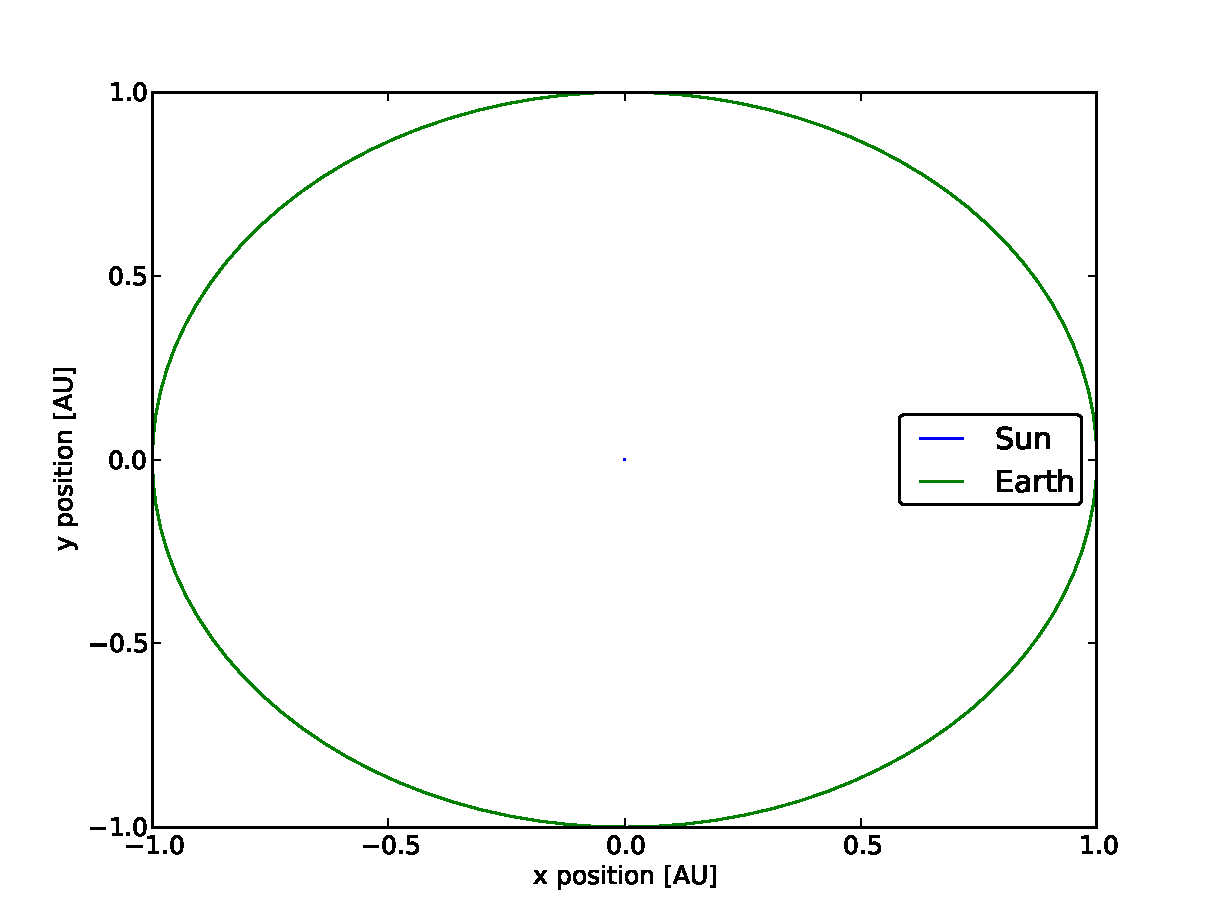
\includegraphics[scale = 0.5]{Fig1.pdf}
\caption{Circular orbit of Earth around the Sun}
\end{figure} 

With these values for $t_{max}$ and $N$ the time step is $h = 0.01$ i.e. 100 points per year (per round). We see that Earth's orbit in this case is stable and smooth. When N is lowered, the number of points per year lowers, and the orbit becomes unstable. For $N = 2000$ there are only 20 points per year and the plot shows that Earth actually moves gradually towards the Sun for every year, which means that RK4 produce wrong results taking into mind that Earth' orbit should be a stable circle for these initial conditions. For $N = 1500$ the plot shows that Earth actually escapes the Sun's gravity well as shown in Figure 2. This is due to the fact that when Earth moves this close to the Sun, the forces becomes so enormous that Earth actually gets pushed away from the Sun. 

\begin{figure}[!h]
\centering
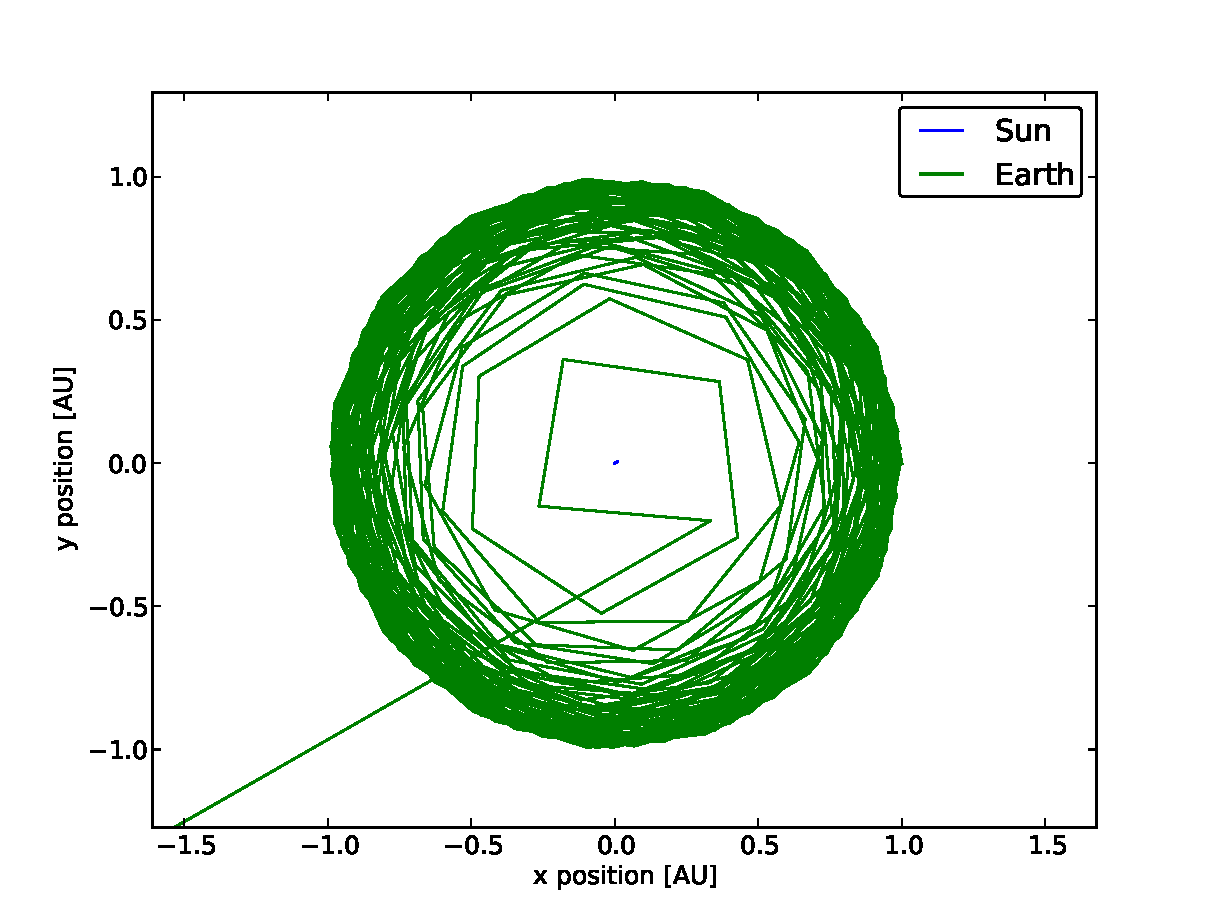
\includegraphics[scale = 0.5]{Fig2.pdf}
\caption{Earth escapes the Sun's gravity well for $N=1500$}
\end{figure} 

A good way to validate the results is to check whether Earth's kinetic and potential energy as well as angular momentum is constant for the case of a circular orbit. When Earth moves in a circle its tangential speed and orbital radius doesn't change, thus it's kinetic and potential energy shouldn't change either. Furthermore, angular momentum is conserved when there is no external torque acting on a system, as is the case for the Earth-Sun system. The functions $kin_energy$, $pot_energy$ and $ang_mom$ in $main.cpp$ calculates these quantities for each time step and writes them to a file for plotting. The result is shown in Figure 3, where we can see that all the quantities oscillate with a peak-to-peak value of about $10^{-5}$, thus they're constant to an approximation of that order.

\begin{figure}[!h]
\centering
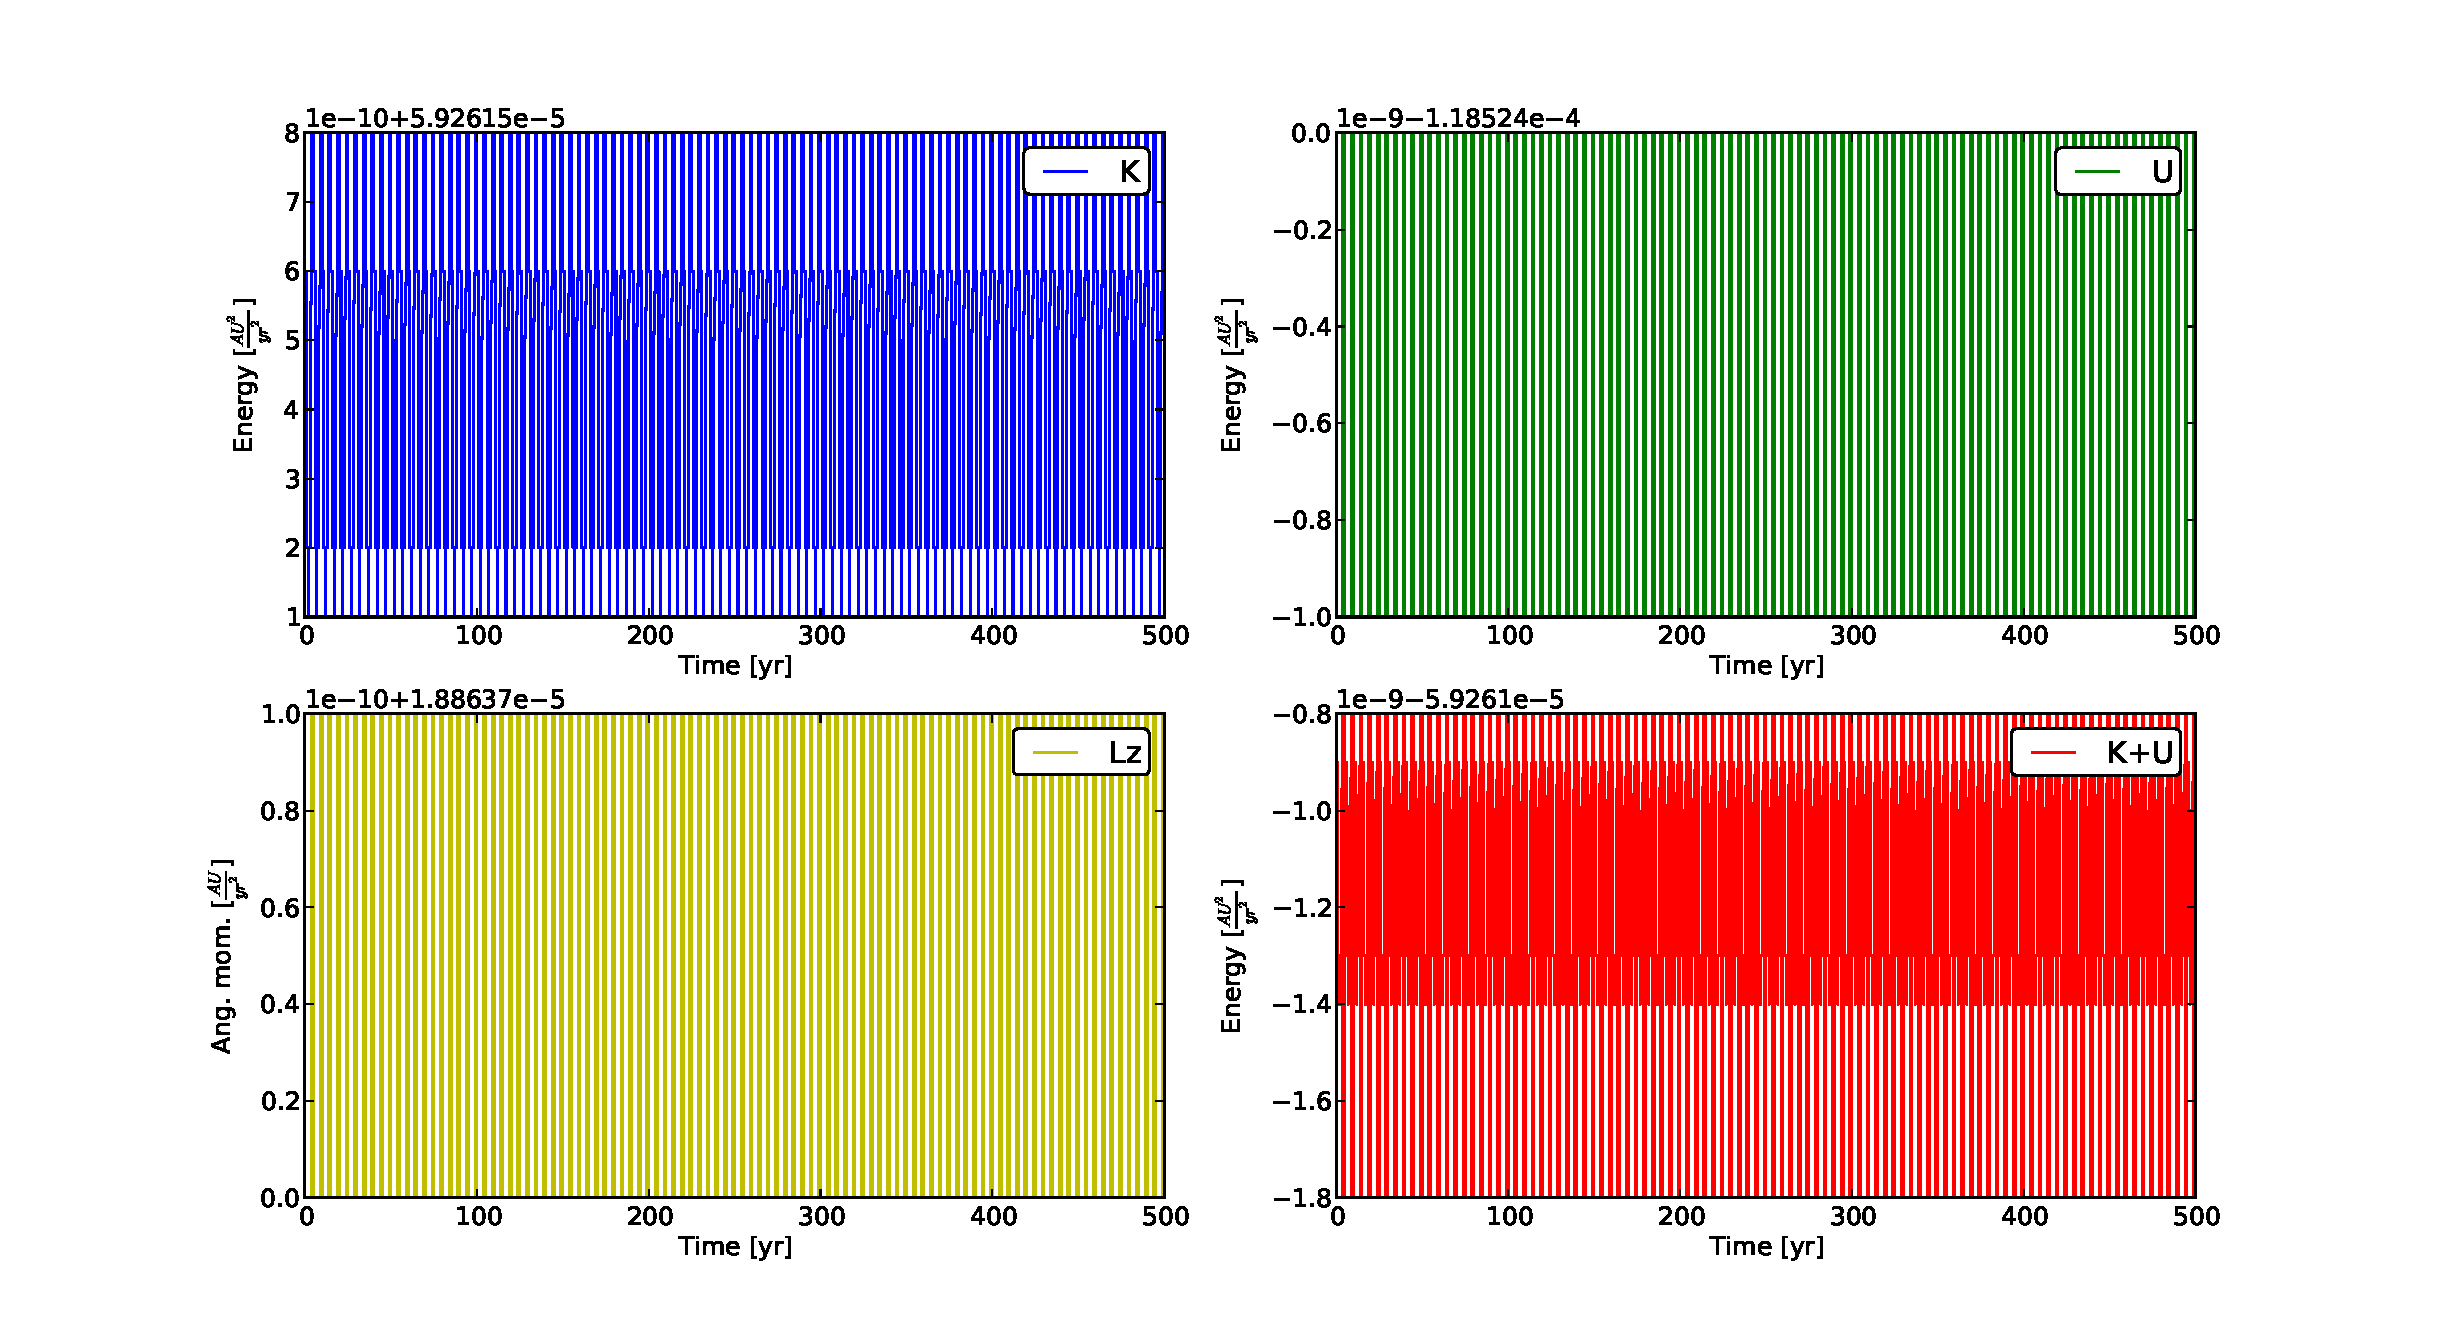
\includegraphics[scale = 0.5]{Fig3.pdf}
\caption{Kinetic energy K, potential energy U, angular momentum Lz and total energy K+U for $N=50000$}
\end{figure} 

\subsection*{Escape velocity}
Testing escape velocity is another good way to validate the results. For a planet in the gravitational field of the Sun, the escape velocity is independent of the planet's mass and is given in closed-form as
\[
v_e = \sqrt{\frac{2GM_{Sun}}{r}}
\]
In units of AU and solar mass for a planet at a distance of 1 AU the velocity is
\[
v_e = \sqrt{2x4\pi^2} AU/yr = \sqrt{8}\pi AU/yr \approx 2.8284\pi AU/yr
\]
This value corresponds very well with my simulation. When I set the initial velocity of the Sun to zero and $v_{y0} = 2.82\pi$ for Earth ($t_max = 500$ and $N = 50000$), it's orbit has a large eccentricity, see Figure 4. When $v_{y0} = 2.84$ however, Earth escapes and moves a long distance away, see Figure 5. This is a good validation of my code. 

\begin{figure}[!h]
\centering
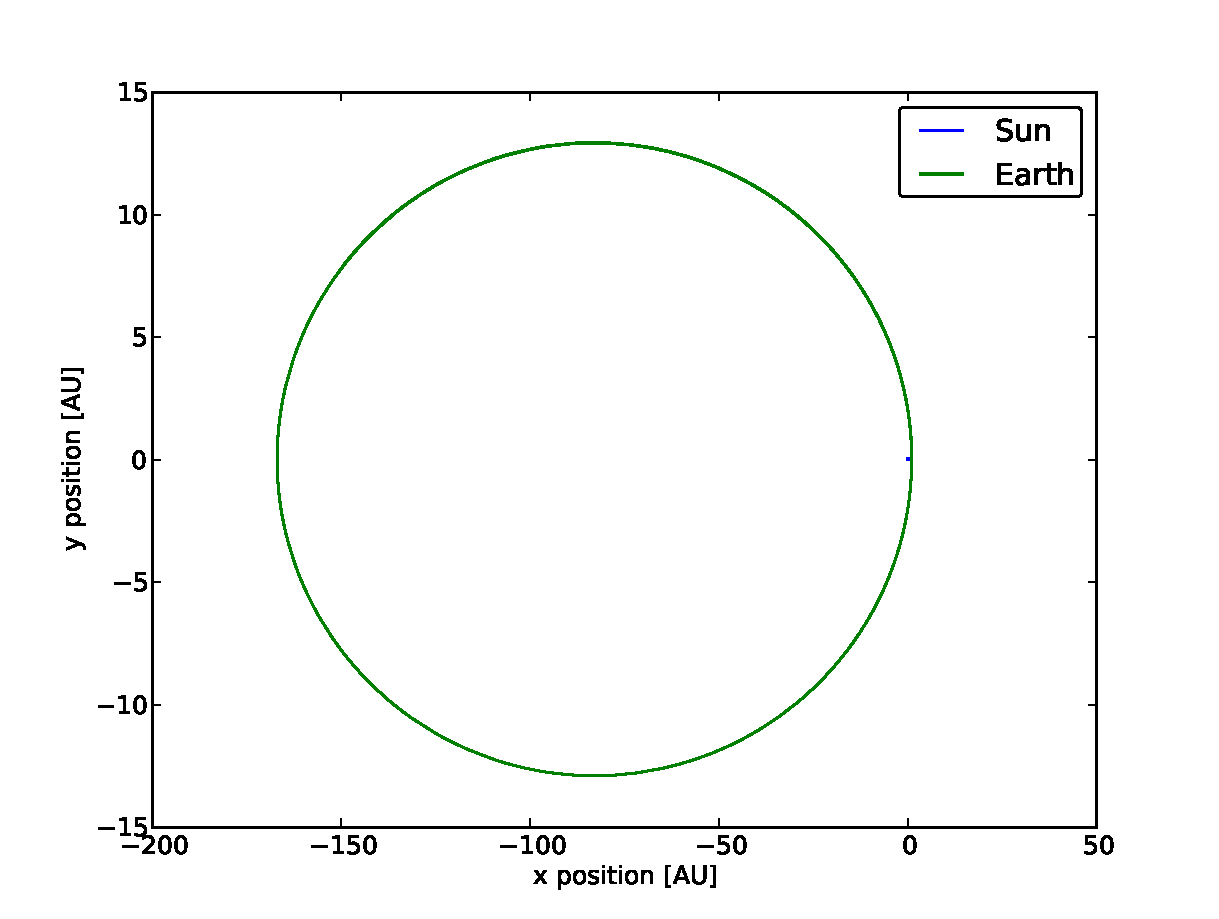
\includegraphics[scale = 0.5]{Fig4.pdf}
\caption{Earth's orbit has a large eccentricity when it's velocity is nearly the escape velocity}
\end{figure} 

\begin{figure}[!h]
\centering
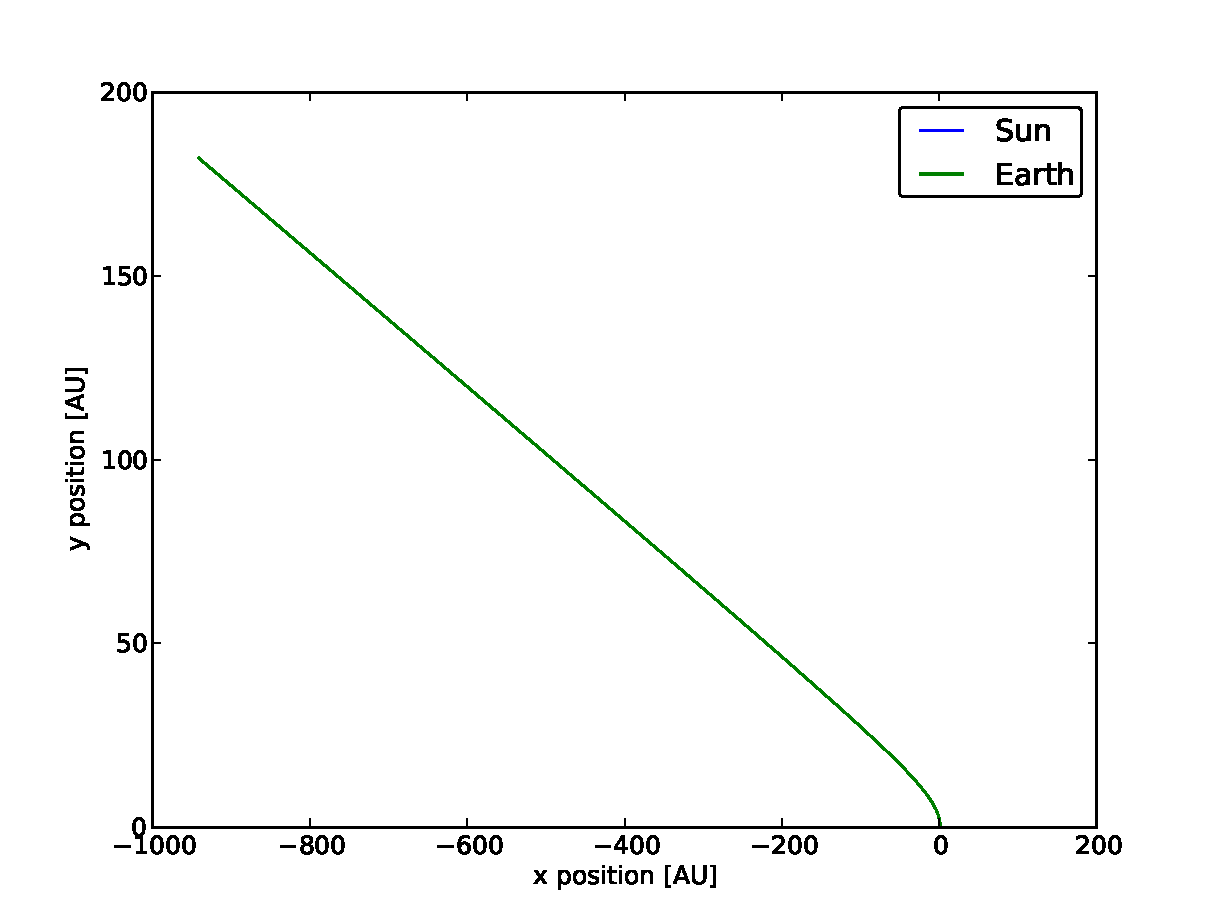
\includegraphics[scale = 0.5]{Fig5.pdf}
\caption{Earth escapes when $v_{y0} = 2.84$}
\end{figure} 

\section*{Three-body problem Sun-Earth-Jupiter}
When adding Jupiter we have a three-body problem, thus the equations of motion have to be generalized. The differential equations for this system is similar to those for the two-body problem, except that we now have to sum the gravitational contribution from all the other objects in the system to compute the acceleration of the object we're looking at. Thus the equations for the x-component of position and velocity for planet $i$ becomes
\[
\frac{dx_i}{dt}=v_{xi} 
\]
and
\[
\frac{d^2x_i}{dt^2}=\frac{dv_{xi}}{dt}=G\sum_{j=0}^n \frac{M_j(x_i-x_j)}{M_{r_{ij}^3}}
\]
where $M_j$ is the mass of object $j$ and $r_{ij}$ is the distance between object $i$ and $j$. This means that the equations can have the same form as before in my program, but now they need to be in a for-loop. This is the general formulas for n objects, for the three-body problem $n=2$. I set up the system in the same way as I did before for Earth and the Sun. I use data for Jupiter from $http://nssdc.gsfc.nasa.gov/planetary/factsheet/index.html$, where I compare Jupiter's values for average orbital velocity and average distance from the Sun to the same quantities for Earth. I set $v_{y0}$ and $x_0$ for Jupiter to these relative values, making it unnecessary to actually convert the values to the correct units. Using these average values should lead to a circular orbit, as shown in figure 6. 

\begin{figure}[!h]
\centering
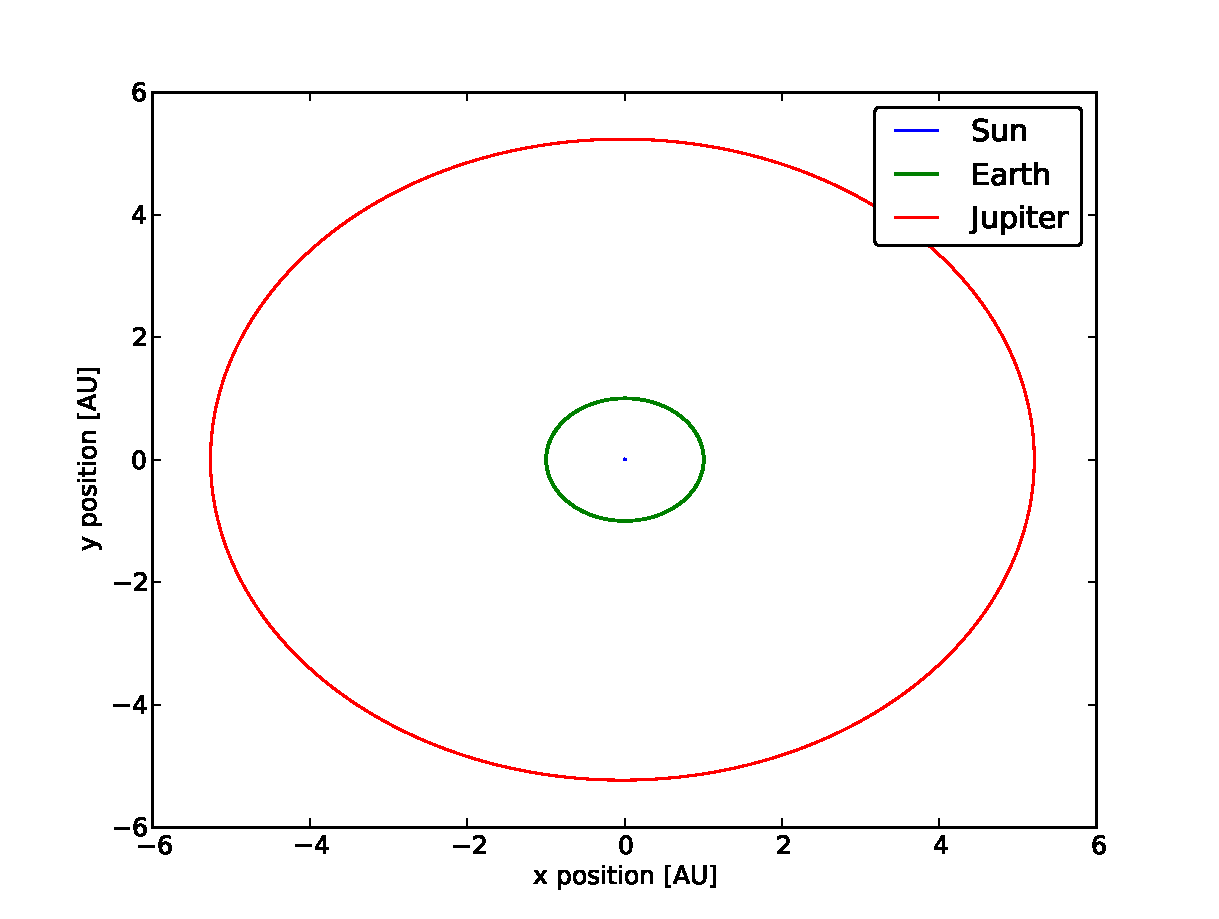
\includegraphics[scale = 0.5]{Fig6.pdf}
\caption{Three-body system Earth-Sun-Jupiter. $t_{max} = 500$ and $N = 50000$}
\end{figure} 

The stability of the RK4 algorithm for this system is about the same as for the two-body problem. It works well for 100 points per year as shown in figure 6, but for 20 points per year the system is no longer stable and Earth escapes as it did in the two-body system (Figure 7). Although Jupiter stays in orbit, we see from the thickness of the red line that it's orbit is quite unstable. However, Earth actually has a more stable (peak-to-peak about $10^{-7}$) energy and angular momentum after the addition of Jupiter when there are 100 points per year (Figure 8), which suggests a better stability for additional objects.

\begin{figure}[!h]
\centering
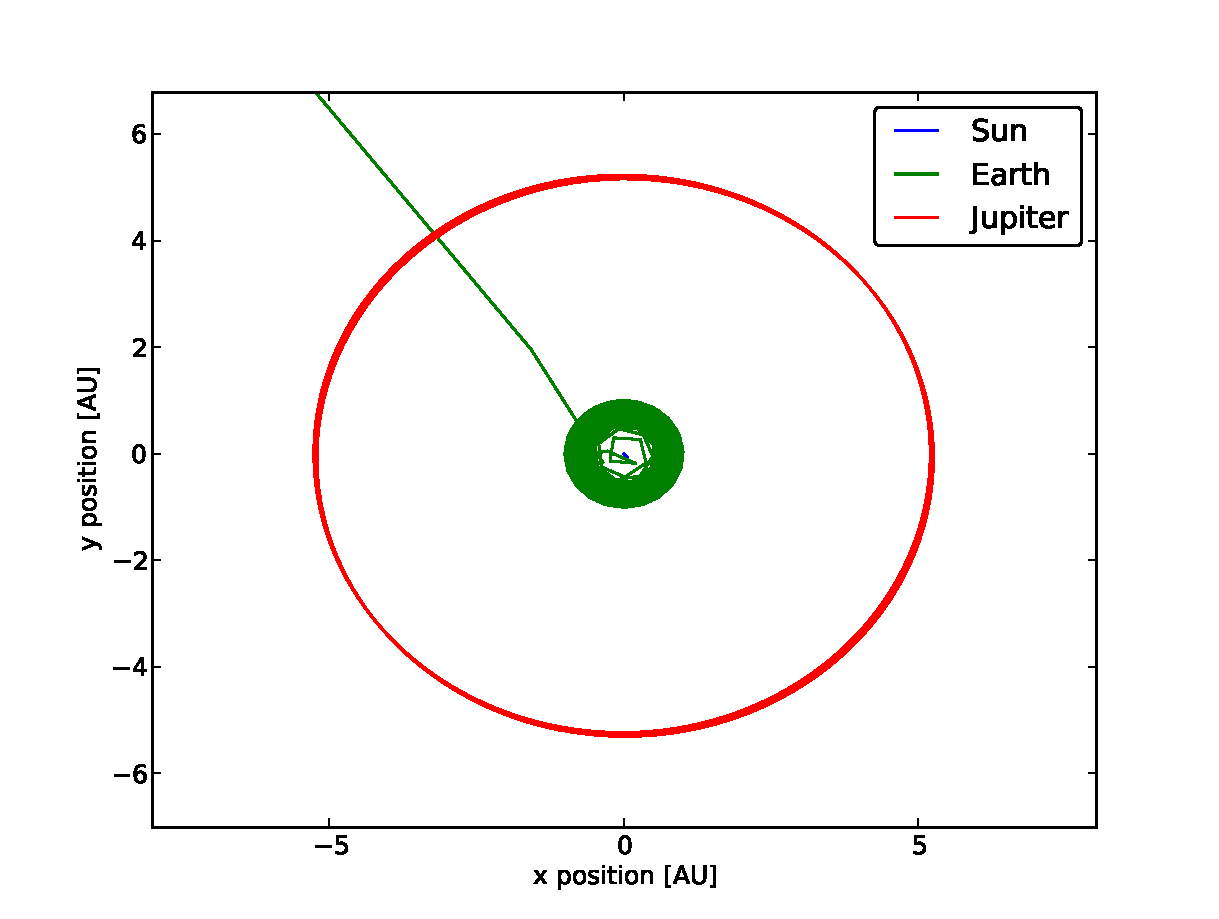
\includegraphics[scale = 0.5]{Fig7.pdf}
\caption{Earth escapes as in the two-body system. $t_{max} = 500$ and $N = 10000$}
\end{figure} 

\begin{figure}[!h]
\centering
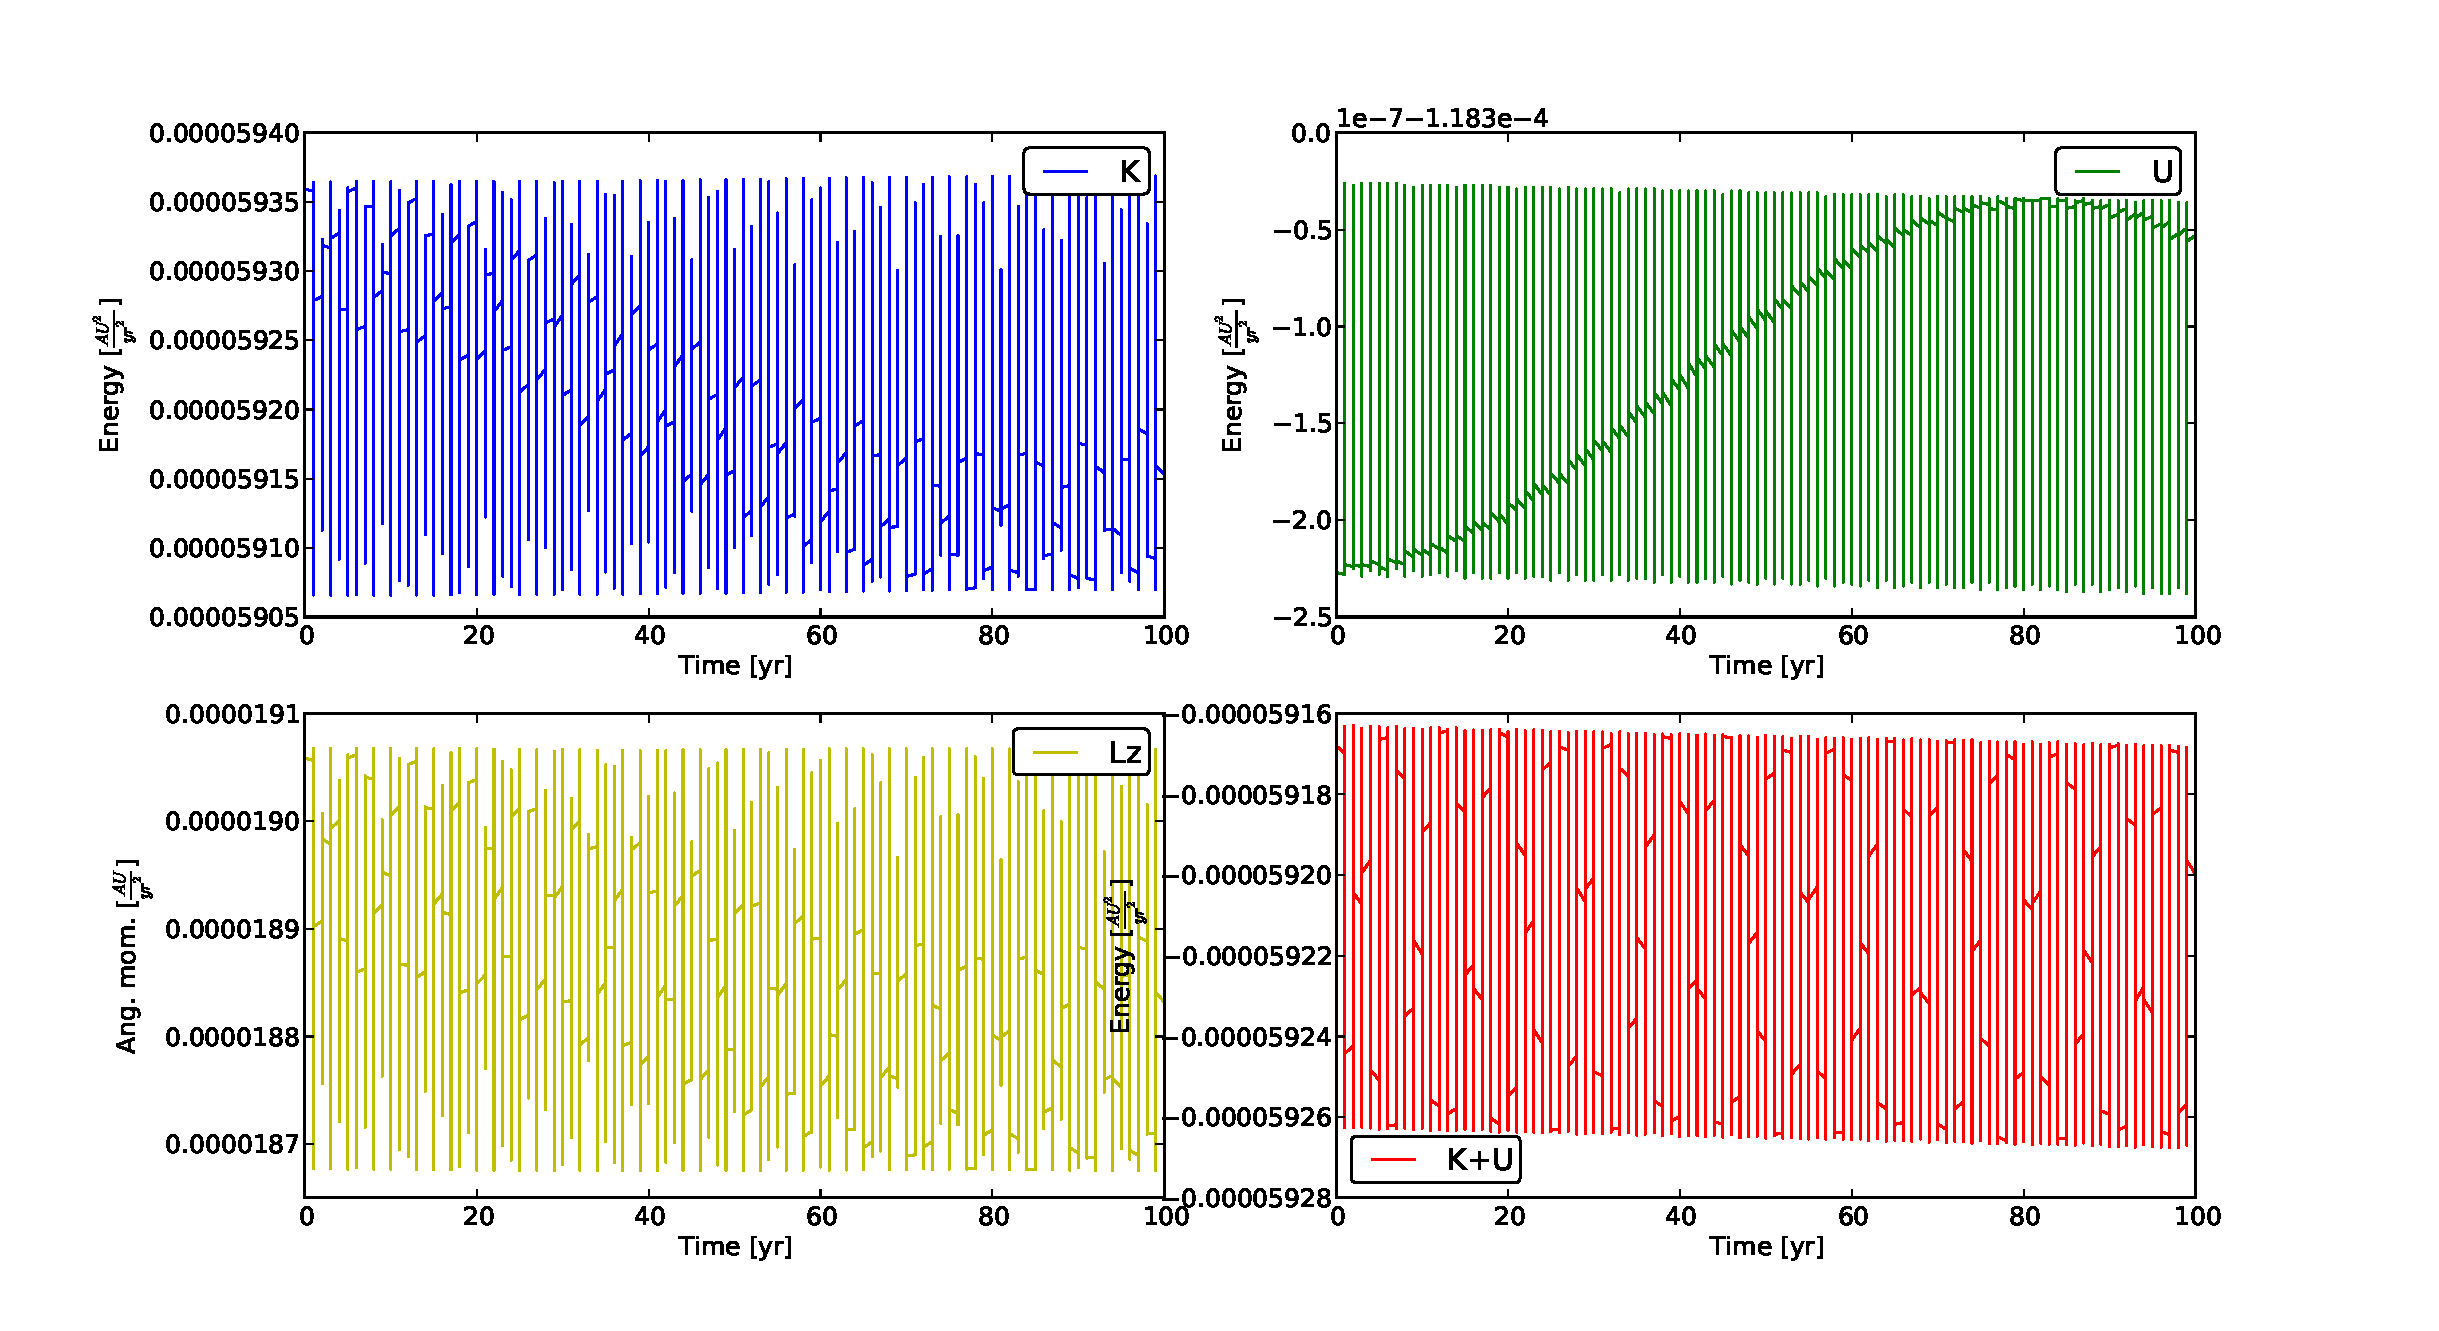
\includegraphics[scale = 0.3]{Fig8.pdf}
\caption{Energy and angular momentum oscillates less after the addition of Jupiter $t_{max} = 500$ and $N = 50000$}
\end{figure} 

Increasing the mass of Jupiter by a factor of 10 reduces the stability only a little; the energy of Earth now oscillates in the order of $10^{-7}$. Increasing the mass by a factor of 1000 however, destabilizes the system drastically. Now Jupiter has about the same mass as the Sun, meaning that Earth suddenly finds itself between two quite massive stars. All three objects go out of orbit in this case (Figure 9), even when there are 1000 points per year, suggesting that this isn't a result of the loss of stability by RK4, but an intrinsic property of the system itself. 

\begin{figure}[!h]
\centering
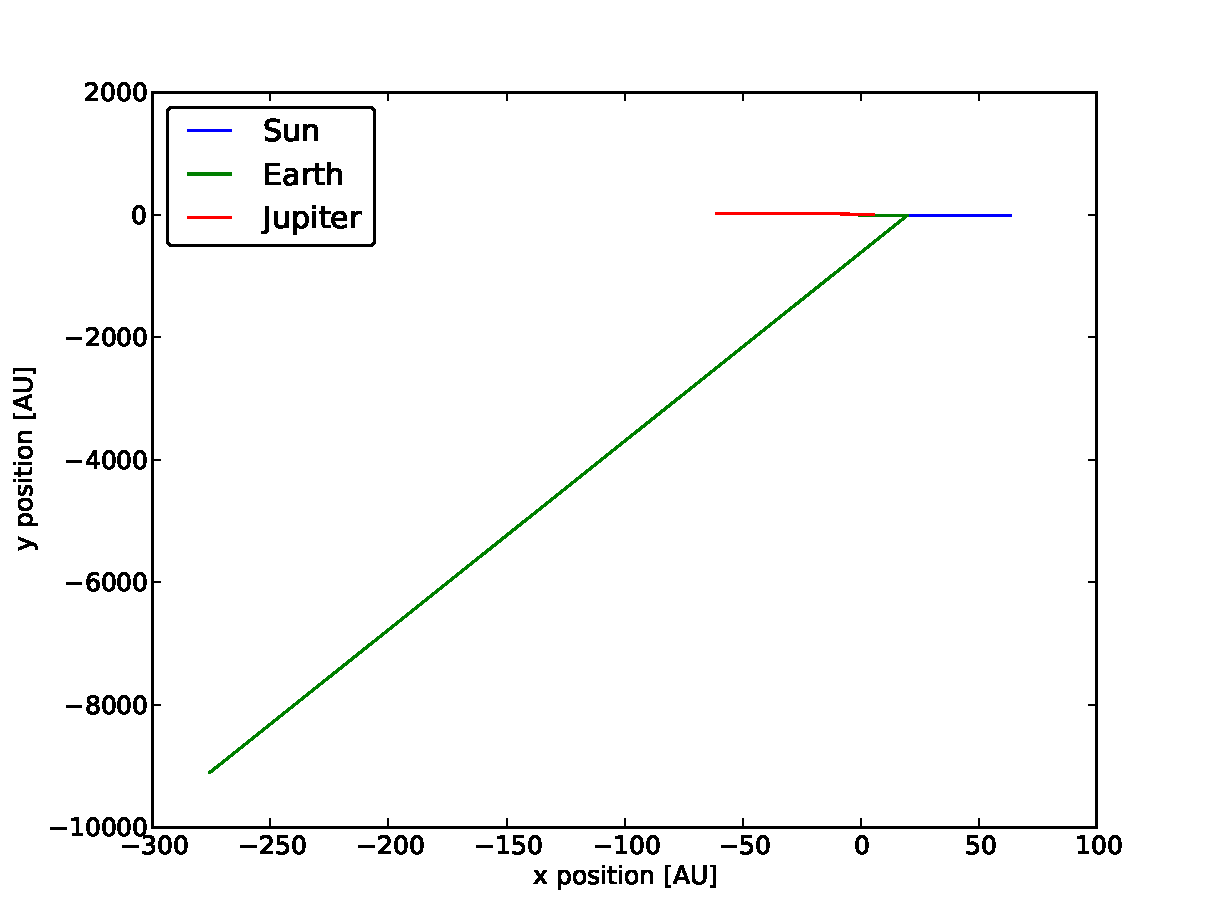
\includegraphics[scale = 0.5]{Fig9.pdf}
\caption{The whole system collapses when Jupiter is as heavy as the Sun}
\end{figure} 

\section*{The Solar System}
I generalized the system for $n$ bodies in the last section, so all I have to do to add the rest of the planets is to make a class object for each of them and set $n = 10$. I set the initial velocity for each planet in the same way as for Jupiter. This makes the orbits of all the planets circular, which is a good approximation except for Pluto, which has a much more elliptical orbit. A larger eccentricity can be achieved by lowering or increasing Pluto's initial velocity while not exceeding it's escape velocity. I have however not been able to find data that fits better.

\begin{figure}[!h]
\centering
\includegraphics[scale = 0.5]{Fig10.pdf}
\caption{Simulation of the whole Solar system. $N = 75000$, $t_{max} = 500$.}
\end{figure} 

RK4 doesn't do the job as well when all the planets are included. The big problem is Mercury, which escapes the system even for 100 points per year because it gets too close to the Sun. For 150 points per year, the system is stable though, as shown in Figure 10. 

\section*{Conclusion}
We've seen in this project that the theoretical basis for simulating the Solar system is simple; only Newton's gravitational law is important. The data flow in the program is more challenging though. I chose to initialize a class object for each planet which save the initial conditions and mass. This class could have been expanded and used to store also the following values etc., so that the object-orientation would have been more distinct. I could also have made a solver class which contained the Runge-Kutta routine and the f function to shorten the main program, but I did not have the time.

The RK4 solver worked relatively well for this problem, although it did get a bit unstable for the whole solar system. A time step of 0.01 was sufficient for the two- and three-body system, but not for the whole deal. The results were validated by checking whether they were consistent with conservation of energy / angular momentum and the closed-form expression of escape velocity. 

\section*{Program listing}
My source files can be found at https://github.com/johnands/Project3.
The main program is $main.cpp$ while $planet.cpp$ contains the Planet class. $constants.cpp$ holds a few global constants. I've used $plot3.py$ to visualize the simulation. 

\end{document}
